El problema que se nos presenta es, dados $k$ vectores ordenados de menor a mayor,
cada uno con $n$ elementos, combinarlos en un único vector con todos los elementos
ordenados de la misma manera. Al igual que antes, presentamos una solución obvia y
otra empleando un algoritmo Divide y Vencerás. 

\subsection{Caso obvio}

En este caso una alternativa es ir iterando sobre cada vector, añadiendo los elementos
del vector de forma ordenada sobre un acumulador. Ello queda ilustrado en la figura
\ref{fig:2a-obvio}, donde primero se unen los vectores que están en rojo y morado para,
a continuación, unir ese resultado con el vector en verde, dando como resultado
un vector global ordenado. 

\begin{figure}
    \centering
    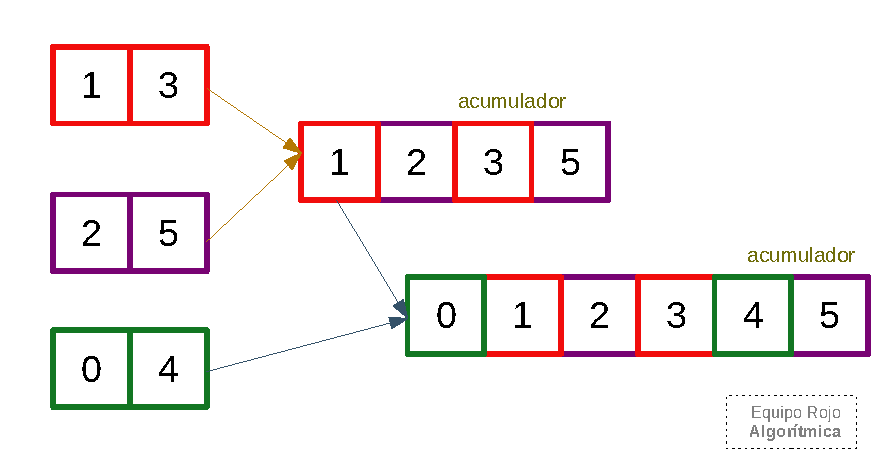
\includegraphics[scale=0.87]{img/orden_2a.pdf}
    \caption{Esquema de funcionamiento del algoritmo de 
    mezcla obvio. Elaboración propia.}
    \label{fig:2a-obvio}
\end{figure}

\subsubsection{Pseudocódigo}

\lstinputlisting[caption=Pseudocódigo asociado a la mezcla 
ordenada de vectores ordenados en el caso obvio., 
label={alg:2a-obvio}]{listing/ejer2a-pseudo-obvio.txt}

\subsubsection{Implementación}

\lstinputlisting[firstline=81, lastline=130, language=C++,
caption=Implementación del algoritmo \ref{alg:2a-obvio}.]{../src/ejercicio-2-mezcla.cpp}

\subsubsection{Análisis de Eficiencia}

En primer lugar, analizamos la \textbf{eficiencia teórica}. En este caso,
el tamaño del problema depende tanto del número de componentes
de los vectores $n$ como del número de vectores $k$ que hemos
considerado. 

Analizando el algoritmo auxiliar UNIFICA de \ref{alg:2a-obvio}, tenemos que el 
número de operaciones que se realiza es independiente
del número de vectores $k$ a considerar, por lo que queda
acotada por una constante. Por su parte, el número de componentes de los
vectores sí influye en el número de operaciones, pues en el ciclo while se recorre completamente
el uno de los vectores y parcialmente la otra, siendo las restantes componentes recorridas
a continuación, por lo que se realizan $cn$ operaciones elementales,
con $c \in \mathbb N$ constante. 

Notemos que el número de operaciones que
se realizan es independiente de los valores de los vectores,
por lo que el mejor caso y el peor caso tienen el mismo orden
de eficiencia. Por tanto, tenemos que su eficiencia es $\theta(n)$. 

% Mal
% \begin{wraptable}{b}{0.3\linewidth}
\begin{table}
    \footnotesize
    \centering
    \begin{tabular}{|r|r|}
        \hline
        $N$ & $T$ $(ms)$ \\
        \hline
        1 & 0.0078 \\ 
        250000 & 130.4093 \\ 
        500000 & 261.6686 \\ 
        750000 & 413.3990 \\ 
        1000000 & 556.9989 \\ 
        1250000 & 692.7300 \\ 
        1500000 & 794.0190 \\ 
        1750000 & 967.6856 \\ 
        2000000 & 1100.9873 \\ 
        2250000 & 1266.8203 \\ 
        2500000 & 1428.2397 \\ 
        2750000 & 1645.1067 \\ 
        3000000 & 1820.3993 \\ 
        3250000 & 1995.0870 \\ 
        3500000 & 2157.7890 \\ 
        3750000 & 2289.4873 \\ 
        4000000 & 2491.1633 \\ 
        4250000 & 2622.4633 \\ 
        4500000 & 2779.7903 \\ 
        4750000 & 2860.5737 \\ 
        5000000 & 2895.9427 \\ 
        5250000 & 2934.2293 \\ 
        5500000 & 3303.9437 \\ 
        5750000 & 3662.6510 \\ 
        6000000 & 3754.8477 \\ 
        6250000 & 3805.5320 \\ 
        6500000 & 3942.2447 \\ 
        6750000 & 4127.4360 \\ 
        7000000 & 4362.7013 \\ 
        7250000 & 4500.4323 \\ 
        7500000 & 4570.1547 \\ 
        7750000 & 4744.1413 \\ 
        8000000 & 4881.4617 \\ 
        8250000 & 5026.1930 \\ 
        8500000 & 5358.3157 \\ 
        8750000 & 5411.3997 \\ 
        9000000 & 5605.6160 \\ 
        9250000 & 5954.4473 \\ 
        9500000 & 6019.2997 \\ 
        9750000 & 6161.2730 \\ 
        \hline
    \end{tabular}
    \caption{Tiempos de ejecución para el algoritmo \ref{alg:2a-obvio},
    	con k constante.}
    \label{tab:2a-obvio-n}
% \end{wraptable}
\end{table}

\begin{table}
	\footnotesize
	\centering
	\begin{tabular}{|r|r|}
		\hline
		$N$ & $T$ $(ms)$ \\
		\hline
		1 & 0.0014 \\ 
		250 & 9.2893 \\ 
		763 & 81.2408 \\ 
		1276 & 229.0587 \\ 
		1789 & 456.9272 \\ 
		2303 & 763.3462 \\ 
		2816 & 1124.6013 \\ 
		3329 & 1592.2963 \\ 
		3842 & 2146.4227 \\ 
		4355 & 2768.3670 \\ 
		4868 & 3443.9970 \\ 
		5382 & 4242.7217 \\ 
		5895 & 5090.0903 \\ 
		6408 & 5977.8030 \\ 
		6921 & 6940.1510 \\ 
		7434 & 8091.5580 \\ 
		7947 & 9220.7350 \\ 
		8461 & 10382.8967 \\ 
		8974 & 11587.4233 \\ 
		9487 & 12911.8067 \\ 
		10000 & 14408.3200 \\ 
		\hline
	\end{tabular}
	\caption{Tiempos de ejecución para el algoritmo 
		\ref{alg:2a-obvio}, con n constante.}
	\label{tab:2a-obvio-k}
\end{table}

Para el algoritmo AGRUPA de \ref{alg:2a-obvio}, que es el que nos interesa,
tenemos que cada iteración del bucle realiza $an + b$, con $a,b \in \mathbb N$ constantes,
operaciones adicionales respecto al anterior,
realizándose un total de $k$ iteraciones. Por tanto, llamando $T(n)$ al número de
operaciones elementales realizadas por el algoritmo, obtenemos la 
expresión \ref{eq:2a-eficiencia}. 

\begin{equation} \label{eq:2a-eficiencia}
    \begin{split}
        T(n) & = (an + b) + 2(an + b) + 3(an + b) + \cdots + k(an + b) \\
             & = (an + b)\sum_{j=1}^k j = (an + b) \frac{k(k+1)}{2} \Rightarrow \boxed{T(n) \in O(nk^2)}
    \end{split}
\end{equation}

Para la \textbf{eficiencia híbrida}, se han tomado dos series de datos pues la eficiencia depende de 2 parámetros.
De esta manera, manteniendo $k$ constante se ha obtenido la tabla \ref{tab:2a-obvio-n}. 
Para $n$ constante, obtenemos la tabla ??. 

En la gráfica \ref{fig:2a-obvio-graph} hemos representado los puntos experimentales con k constante, 
así como la función
de ajuste lineal asociada, con \textbf{función de ajuste} $f$ y \textbf{coeficiente de regresión}
$R^2$ especificada en \ref{eq:2a-ajuste-n}. 

\begin{equation}
    \boxed{f(n) = 6,0739 \cdot 10 ^{-4}  n + 0,9924, R^2 = 0,9978}
    \label{eq:2a-ajuste-n}
\end{equation}

\begin{equation}
\boxed{f(k) = 1,4158 \cdot 10^{-4} \cdot k^2 + 0,0294 k + 0,0219, R^2 = 0,9989}
\label{eq:2a-ajuste-k}
\end{equation}

\begin{figure}
    \centering
    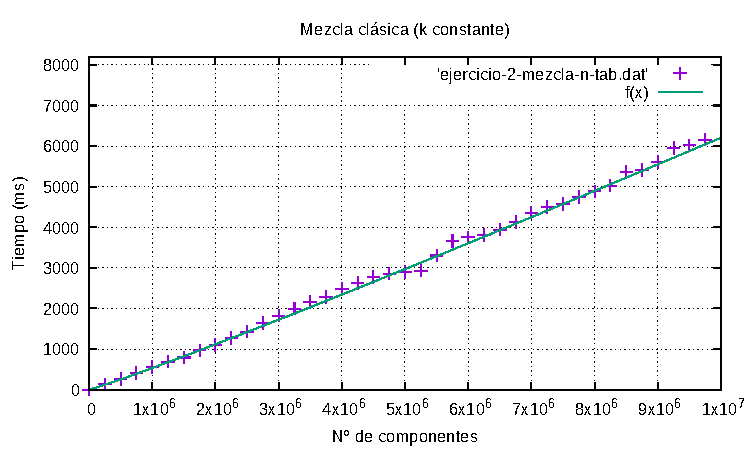
\includegraphics[scale=0.76]{img/e2a-graph.pdf}
    \caption{Gráfica de tiempos de ejecución para el caso obvio, 
    con f(x) y coeficiente de regresión especificada por \ref{eq:2a-ajuste}.}
    \label{fig:2a-obvio-n-graph}
\end{figure}

\begin{figure}
	\centering
	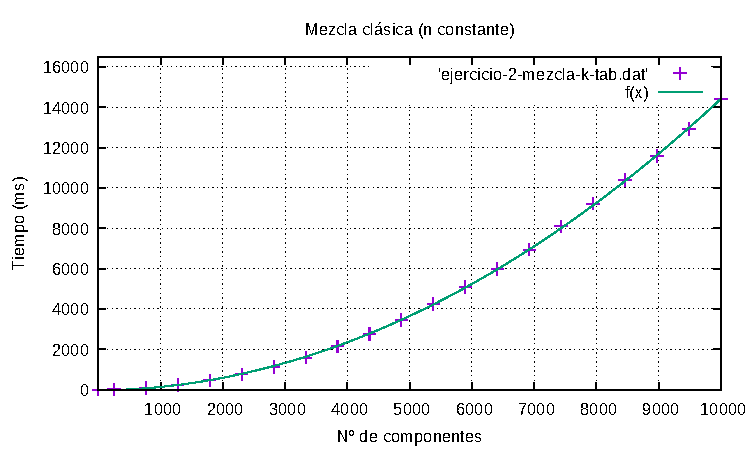
\includegraphics[scale=0.76]{img/e2-obvio-k.pdf}
	\caption{Gráfica de tiempos de ejecución para el caso obvio con n constante, 
		con f(x) y coeficiente de regresión especificada por \ref{eq:2a-ajuste-k}.}
	\label{fig:2a-obvio-k-graph}
\end{figure}